
La premi�re partie est de consuitre les topologies virtualis�es et de
tester les performances de MTPCP en faisant varier les param�tres des
sous-flots. La seconde partie est de construire un alogrithme
d'ordonnancement r�pondant � des crit�res de s�curit�.
\vspace{0.5cm}

Les �tapes du d�veloppement suivront les points suivants:

\begin{itemize}
\item Pr�paration d'une machine mininet avec le noyau MPTCP compil�
  pour l'ensemble de l'�quipe:
\item Lecture, compr�hension et commentaires du code de MPTCP;
\item Pr�paration de plusieurs topologies : \emph{fat tree} pour
  simuler un \emph{data center} et une topologie permettant de tester
  la concurrence entre MPTCP et TCP;
\item Pr�paration d'une biblioth�que de tests et de mesures via l'API python;
\item \'Ecriture d'un algorithme d'ordonnancement dans le noyau;
\item Mesures de performance des diff�rents algorithmes.
\end{itemize}



\subsection{Descriptif du travail de Quentin Dubois et de Kevin Lam}
\begin{figure}[!htb]
  \begin{changemargin}{-2.0cm}{0.5cm}
    \centering
    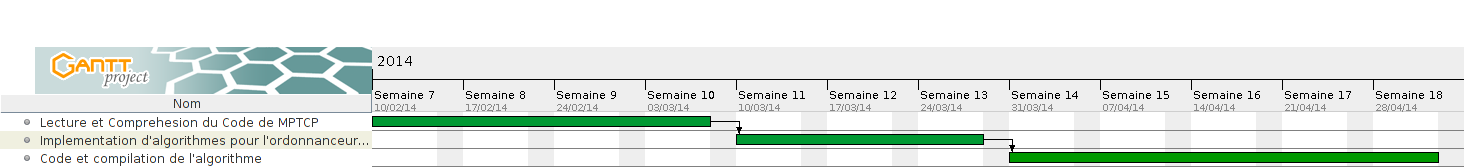
\includegraphics[width=1.2\textwidth]{../gantt/Kevin et Quentin.png}
  \end{changemargin}
  \centering
  
  \caption{\textbf{Diagramme de Gantt Kevin Lam et Quentin Dubois}. }
  \label{fig:gantt}
\end{figure}




\vspace{2cm}
\clearpage
\subsection{Descriptif du travail de Romain Ly}
\begin{figure}[!htb]
  \begin{changemargin}{-2.0cm}{0.5cm}
    \centering
    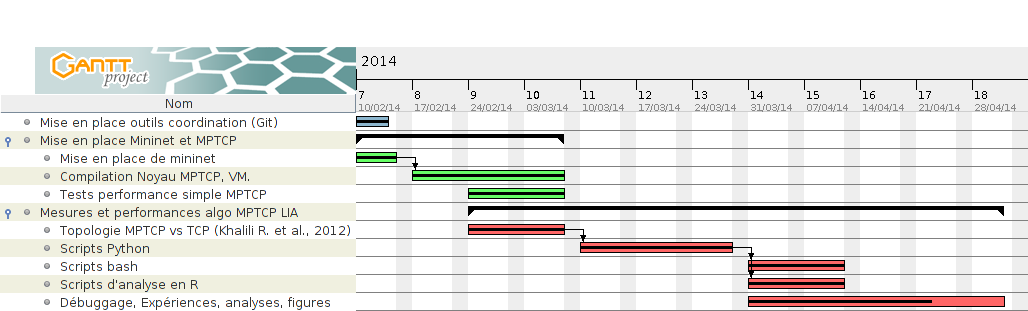
\includegraphics[width=1.2\textwidth]{../gantt/romain.png}
  \end{changemargin}
  \centering
  
  \caption{\textbf{Diagramme de Gantt de Romain Ly.}}
  \label{fig:gantt}
  
\end{figure}
Mise en place du Git
Compilation noyau MPTCP dans la VM mininet et tests simples de routines
Topologie modifi�e de Khalili et al.
Scripts Python
   - impl�mentation d'un parseur d'arguments
   - int�gration de ping, iperf, bwm-ng, sshd, tcpdump permettant le monitoring et l'�tude du r�seau
Installation de TCP-reduce dans la VM pour v�rifier les options de la connexion TCP.
Scripts Bash pour g�n�rer de multiples simulations par l'interm�diaire de scripts Python
Scripts R pour analyse des r�sultats et figures
D�bogages des scripts
Exp�rimentations avec des liens isotropiques
   - variation du nombre de sous flots, d�bit, latence

\subsection{Descriptif du travail de Simon Ravier}

\begin{figure}[!htb]
  \begin{changemargin}{-2.0cm}{0.5cm}
    \centering
    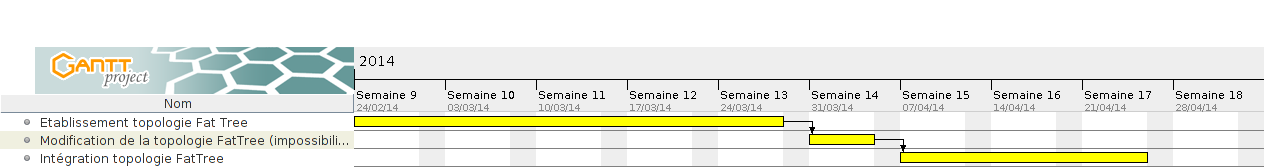
\includegraphics[width=1.2\textwidth]{../gantt/Simon.png}
  \end{changemargin}
  \centering
  
  \caption{\textbf{Diagramme de Gantt de Simon Ravier.}}
  \label{fig:gantt}
\end{figure}

\vspace{1cm}
\begin{tabular}{lp{12cm}}
  03/03 au 30/03 & �tablissement de la topologie FatTree\\
  31/03 au 06/04 & modification de la topologie FatTree (impossibilit� technique de r�aliser le premier mod�le)\\
  07/04 au 27/04 & Int�gration de la topologie FatTree dans
l'environnement de tests (configuration des h�tes, �tablissement des
tables de routage) et r�alisation des tests
\end{tabular}
\vspace{0.5cm}